% Options for packages loaded elsewhere
% Options for packages loaded elsewhere
\PassOptionsToPackage{unicode}{hyperref}
\PassOptionsToPackage{hyphens}{url}
\PassOptionsToPackage{dvipsnames,svgnames,x11names}{xcolor}
%
\documentclass[
  11pt,
  letterpaper,
]{article}
\usepackage{xcolor}
\usepackage[margin=1in]{geometry}
\usepackage{amsmath,amssymb}
\setcounter{secnumdepth}{5}
\usepackage{iftex}
\ifPDFTeX
  \usepackage[T1]{fontenc}
  \usepackage[utf8]{inputenc}
  \usepackage{textcomp} % provide euro and other symbols
\else % if luatex or xetex
  \usepackage{unicode-math} % this also loads fontspec
  \defaultfontfeatures{Scale=MatchLowercase}
  \defaultfontfeatures[\rmfamily]{Ligatures=TeX,Scale=1}
\fi
\usepackage{lmodern}
\ifPDFTeX\else
  % xetex/luatex font selection
\fi
% Use upquote if available, for straight quotes in verbatim environments
\IfFileExists{upquote.sty}{\usepackage{upquote}}{}
\IfFileExists{microtype.sty}{% use microtype if available
  \usepackage[]{microtype}
  \UseMicrotypeSet[protrusion]{basicmath} % disable protrusion for tt fonts
}{}
\makeatletter
\@ifundefined{KOMAClassName}{% if non-KOMA class
  \IfFileExists{parskip.sty}{%
    \usepackage{parskip}
  }{% else
    \setlength{\parindent}{0pt}
    \setlength{\parskip}{6pt plus 2pt minus 1pt}}
}{% if KOMA class
  \KOMAoptions{parskip=half}}
\makeatother
% Make \paragraph and \subparagraph free-standing
\makeatletter
\ifx\paragraph\undefined\else
  \let\oldparagraph\paragraph
  \renewcommand{\paragraph}{
    \@ifstar
      \xxxParagraphStar
      \xxxParagraphNoStar
  }
  \newcommand{\xxxParagraphStar}[1]{\oldparagraph*{#1}\mbox{}}
  \newcommand{\xxxParagraphNoStar}[1]{\oldparagraph{#1}\mbox{}}
\fi
\ifx\subparagraph\undefined\else
  \let\oldsubparagraph\subparagraph
  \renewcommand{\subparagraph}{
    \@ifstar
      \xxxSubParagraphStar
      \xxxSubParagraphNoStar
  }
  \newcommand{\xxxSubParagraphStar}[1]{\oldsubparagraph*{#1}\mbox{}}
  \newcommand{\xxxSubParagraphNoStar}[1]{\oldsubparagraph{#1}\mbox{}}
\fi
\makeatother


\usepackage{longtable,booktabs,array}
\newcounter{none} % for unnumbered tables
\usepackage{calc} % for calculating minipage widths
% Correct order of tables after \paragraph or \subparagraph
\usepackage{etoolbox}
\makeatletter
\patchcmd\longtable{\par}{\if@noskipsec\mbox{}\fi\par}{}{}
\makeatother
% Allow footnotes in longtable head/foot
\IfFileExists{footnotehyper.sty}{\usepackage{footnotehyper}}{\usepackage{footnote}}
\makesavenoteenv{longtable}
\usepackage{graphicx}
\makeatletter
\newsavebox\pandoc@box
\newcommand*\pandocbounded[1]{% scales image to fit in text height/width
  \sbox\pandoc@box{#1}%
  \Gscale@div\@tempa{\textheight}{\dimexpr\ht\pandoc@box+\dp\pandoc@box\relax}%
  \Gscale@div\@tempb{\linewidth}{\wd\pandoc@box}%
  \ifdim\@tempb\p@<\@tempa\p@\let\@tempa\@tempb\fi% select the smaller of both
  \ifdim\@tempa\p@<\p@\scalebox{\@tempa}{\usebox\pandoc@box}%
  \else\usebox{\pandoc@box}%
  \fi%
}
% Set default figure placement to htbp
\def\fps@figure{htbp}
\makeatother


% definitions for citeproc citations
\NewDocumentCommand\citeproctext{}{}
\NewDocumentCommand\citeproc{mm}{%
  \begingroup\def\citeproctext{#2}\cite{#1}\endgroup}
\makeatletter
 % allow citations to break across lines
 \let\@cite@ofmt\@firstofone
 % avoid brackets around text for \cite:
 \def\@biblabel#1{}
 \def\@cite#1#2{{#1\if@tempswa , #2\fi}}
\makeatother
\newlength{\cslhangindent}
\setlength{\cslhangindent}{1.5em}
\newlength{\csllabelwidth}
\setlength{\csllabelwidth}{3em}
\newenvironment{CSLReferences}[2] % #1 hanging-indent, #2 entry-spacing
 {\begin{list}{}{%
  \setlength{\itemindent}{0pt}
  \setlength{\leftmargin}{0pt}
  \setlength{\parsep}{0pt}
  % turn on hanging indent if param 1 is 1
  \ifodd #1
   \setlength{\leftmargin}{\cslhangindent}
   \setlength{\itemindent}{-1\cslhangindent}
  \fi
  % set entry spacing
  \setlength{\itemsep}{#2\baselineskip}}}
 {\end{list}}
\usepackage{calc}
\newcommand{\CSLBlock}[1]{\hfill\break\parbox[t]{\linewidth}{\strut\ignorespaces#1\strut}}
\newcommand{\CSLLeftMargin}[1]{\parbox[t]{\csllabelwidth}{\strut#1\strut}}
\newcommand{\CSLRightInline}[1]{\parbox[t]{\linewidth - \csllabelwidth}{\strut#1\strut}}
\newcommand{\CSLIndent}[1]{\hspace{\cslhangindent}#1}



\setlength{\emergencystretch}{3em} % prevent overfull lines

\providecommand{\tightlist}{%
  \setlength{\itemsep}{0pt}\setlength{\parskip}{0pt}}



 


\usepackage{booktabs}
\usepackage{longtable}
\usepackage{array}
\usepackage{multirow}
\usepackage{wrapfig}
\usepackage{float}
\usepackage{colortbl}
\usepackage{pdflscape}
\usepackage{tabu}
\usepackage{threeparttable}
\usepackage{threeparttablex}
\usepackage[normalem]{ulem}
\usepackage{makecell}
\usepackage{xcolor}
\usepackage{authblk}
\AtBeginDocument{\hypersetup{pdfauthor={Jinseob Kim; Taehee Shin}}}
\renewcommand\Affilfont{\normalsize}
\author[1,*]{Jinseob Kim}
\author[1,2]{Taehee Shin}
\affil[1]{Zarathu Co., Ltd., Seoul, South Korea}
\affil[2]{Department of Applied Statistics, Yonsei University, Seoul, South Korea}
\affil[*]{Corresponding author: \protect\href{mailto:jinseob2kim@gmail.com}{jinseob2kim@gmail.com}}
\renewcommand\author[2][]{}
\makeatletter
\@ifpackageloaded{caption}{}{\usepackage{caption}}
\AtBeginDocument{%
\ifdefined\contentsname
  \renewcommand*\contentsname{Table of contents}
\else
  \newcommand\contentsname{Table of contents}
\fi
\ifdefined\listfigurename
  \renewcommand*\listfigurename{List of Figures}
\else
  \newcommand\listfigurename{List of Figures}
\fi
\ifdefined\listtablename
  \renewcommand*\listtablename{List of Tables}
\else
  \newcommand\listtablename{List of Tables}
\fi
\ifdefined\figurename
  \renewcommand*\figurename{Figure}
\else
  \newcommand\figurename{Figure}
\fi
\ifdefined\tablename
  \renewcommand*\tablename{Table}
\else
  \newcommand\tablename{Table}
\fi
}
\@ifpackageloaded{float}{}{\usepackage{float}}
\floatstyle{ruled}
\@ifundefined{c@chapter}{\newfloat{codelisting}{h}{lop}}{\newfloat{codelisting}{h}{lop}[chapter]}
\floatname{codelisting}{Listing}
\newcommand*\listoflistings{\listof{codelisting}{List of Listings}}
\makeatother
\makeatletter
\makeatother
\makeatletter
\@ifpackageloaded{caption}{}{\usepackage{caption}}
\@ifpackageloaded{subcaption}{}{\usepackage{subcaption}}
\makeatother
\usepackage{bookmark}
\IfFileExists{xurl.sty}{\usepackage{xurl}}{} % add URL line breaks if available
\urlstyle{same}
\hypersetup{
  pdftitle={Redefining the Null Hypothesis: Incorporating Uncertainty to Address the Limitations of Traditional p-values},
  pdfkeywords={p-value, effect size, null
hypothesis, uncertainty, hypothesis testing, statistical
significance, equivalence testing},
  colorlinks=true,
  linkcolor={blue},
  filecolor={Maroon},
  citecolor={blue},
  urlcolor={blue},
  pdfcreator={LaTeX via pandoc}}


\title{Redefining the Null Hypothesis: Incorporating Uncertainty to
Address the Limitations of Traditional p-values}
\author{}
\date{November 16, 2026}
\begin{document}
\maketitle
\begin{abstract}
The p-value has a fundamental limitation: with sufficiently large
samples, even trivially small effects become statistically significant,
because most studies test the unrealistic point null hypothesis that the
true effect is exactly zero. We propose a hypothesis testing framework
that incorporates uncertainty into the null hypothesis by replacing the
point null with a normal distribution centered at the null value. The
resulting test statistic is the conventional statistic shrunk by a
factor of \(1/\sqrt{1+nc^2}\), where \(c\) is the standardized
uncertainty, yielding an effect-size-integrated p-value. Simulation
studies show that the test controls the Type I error rate at or below
the nominal level, with exact size under the distributional null and
conservative behavior under the point null. Its minimum detectable
effect converges to approximately \(1.96c\) as the sample size grows, so
effects below this threshold cannot reach significance however large the
sample. We illustrate the approach with data on maternal smoking and
birth weight and compare it with equivalence testing. The framework
incorporates effect size directly into hypothesis testing and offers a
principled way to distinguish statistical from practical significance.
\end{abstract}

\noindent\textbf{Keywords:} p-value; effect size; null hypothesis; uncertainty; hypothesis testing; statistical significance; equivalence testing
\bigskip


\section{Introduction}\label{sec-intro}

Null hypothesis significance testing remains the dominant framework for
scientific claims in the natural and social sciences
(\citeproc{ref-anderson2000null}{Anderson et al. 2000}). Following
Fisher, the p-value quantifies how surprising the observed data would be
if the null hypothesis were true (\citeproc{ref-2528399}{Yates 1964}),
and \(p < 0.05\) has long served as the conventional threshold for
discovery (\citeproc{ref-ronald2016asa}{Wasserstein and Lazar 2016}).
Persistent criticism of this practice has led to proposals such as
lowering the threshold to 0.005 (\citeproc{ref-jama20181536}{Ioannidis
2018}; \citeproc{ref-Benjamin2018}{Benjamin et al. 2018}). These
proposals, however, leave a more basic problem untouched: with a
sufficiently large sample, any nonzero difference becomes statistically
significant.

This problem is now practical rather than theoretical. Studies based on
electronic health records, nationwide health insurance claims databases,
and online platforms routinely analyze hundreds of thousands to millions
of observations. At such sample sizes, p-values for negligible
differences collapse toward zero, and statistical significance carries
little information about whether an effect matters
(\citeproc{ref-lin2013too}{Lin et al. 2013}). For a two-sided z-test
with \(z = (\bar{X} - \mu_0)/(\sigma/\sqrt{n})\), any
\(\bar{X} \neq \mu_0\) yields a p-value that approaches zero as \(n\)
increases.

We identify the point null hypothesis as the root cause. A null
hypothesis must be stated precisely (e.g., \(\mu = 0\)) to be refutable,
but an effect of exactly zero is rarely plausible. Meehl argued that in
the behavioral sciences the point null is almost always false, so that
its rejection becomes nearly certain as the sample grows and offers weak
support for any substantive theory (\citeproc{ref-meehl1967theory}{Meehl
1967}). Cohen likewise observed that the ``nil'' hypothesis of exactly
zero effect is essentially never true in practice, so that rejecting it
is uninformative (\citeproc{ref-cohen1994earth}{Cohen 1994}).
Conventional tests nevertheless treat the null value as known without
error.

This limitation has led to calls for examining effect sizes alongside
p-values (\citeproc{ref-sullivan2012using}{Sullivan and Feinn 2012}).
Effect size, which standardizes the observed difference---typically by
dividing by the standard deviation---is already used in sample size
calculations. Establishing a realistic null hypothesis is not only
important in itself but is also directly connected to considering effect
sizes.

\subsection{Related Work}\label{related-work}

Several approaches have been proposed to address the limitations of
traditional null hypothesis significance testing:

\textbf{Interval null hypotheses.} Hodges and Lehmann proposed testing
whether a parameter lies within a small neighborhood of the null value
rather than exactly at it, on the grounds that point hypotheses are
seldom exactly true (\citeproc{ref-hodges1954testing}{Hodges and Lehmann
1954}). Equivalence testing, minimum-effect testing, and
second-generation p-values can all be viewed as descendants of this
idea; our distributional null is a smooth analog of the interval null.

\textbf{Lindley's paradox.} Lindley showed that, for a fixed p-value,
the posterior probability of a point null hypothesis tends to one as the
sample size grows, so that frequentist and Bayesian conclusions diverge
in large samples (\citeproc{ref-lindley1957statistical}{Lindley 1957}).
Our framework addresses the same large-sample tension from the
frequentist side.

\textbf{Equivalence Testing and TOST.} The Two One-Sided Tests (TOST)
procedure tests whether an effect falls within a pre-specified
equivalence bound \([-\delta, \delta]\), effectively asking whether the
effect is ``practically equivalent to zero'' rather than exactly zero
(\citeproc{ref-lakens2017equivalence}{Lakens 2017}). Our approach shares
this motivation but implements it through a continuous uncertainty
parameter rather than discrete bounds.

\textbf{Second-Generation p-values (SGPV).} Blume et al.~proposed
second-generation p-values that incorporate a null interval rather than
a point null (\citeproc{ref-blume2018second}{Blume et al. 2018}). Our
approach is conceptually similar, replacing the point null with a
distributional assumption that serves as a continuous analog to the null
interval.

\textbf{Region of Practical Equivalence (ROPE).} In Bayesian inference,
the ROPE defines a range of parameter values considered practically
equivalent to the null value
(\citeproc{ref-kruschke2018bayesian}{Kruschke and Liddell 2018}). While
our method operates within a frequentist framework, it shares the
philosophical motivation of distinguishing between statistical and
practical significance.

\textbf{Redefining Statistical Significance.} Benjamin et al.~proposed
lowering the significance threshold to 0.005 to reduce false positive
rates (\citeproc{ref-Benjamin2018}{Benjamin et al. 2018}). However, this
approach does not address the fundamental issue that any fixed threshold
can be overcome with sufficient sample size.

Existing practice typically reports p-values and effect sizes side by
side and leaves their joint interpretation to the reader. In our
framework, the effect size enters the test statistic directly, yielding
a sample-size-adaptive criterion that penalizes trivially small effects.

\subsection{Contributions}\label{contributions}

\begin{enumerate}
\def\labelenumi{\arabic{enumi}.}
\item
  \textbf{Effect-size-integrated p-value:} Introducing standardized
  uncertainty into the null via \(\tau = c\sigma\) shrinks Wald
  statistics by \(1/\sqrt{1+nc^2}\), integrating effect size and sample
  size into a single measure.
\item
  \textbf{Minimum detectable effect and sample size:} The framework
  yields \(\text{MDE}(n) = z_{1-\alpha/2}\sqrt{1/n + c^2}\), which
  bounds significance even as \(n \to \infty\), together with a
  closed-form sample size formula (Section~\ref{sec-samplesize}).
\item
  \textbf{Calibration and interpretation:} The test has exact size
  \(\alpha\) under the distributional null and is conservative under the
  point null, and its rejection region is closely related to the
  interval criteria underlying TOST and SGPV.
\end{enumerate}

The remainder of this paper is organized as follows.
Section~\ref{sec-methods} introduces the uncertainty-adjusted null
hypothesis, derives the shrinkage factor and the minimum detectable
effect, and extends the approach to t, regression, and chi-square
statistics. Section~\ref{sec-results} evaluates Type I error and power
by simulation (Section~\ref{sec-sim}), applies the method to birth
weight data (Section~\ref{sec-real}), and compares it with equivalence
testing (Section~\ref{sec-tost}). Section~\ref{sec-guidelines} gives
practical guidance on choosing \(c\) and on sample size calculation.
Section~\ref{sec-discussion} discusses the relation to Bayesian
approaches, an exploratory extension to multiple testing, and
limitations, and Section~\ref{sec-conclusion} concludes.

\section{Materials and Methods}\label{sec-methods}

\subsection{Null Hypothesis with
Uncertainty}\label{null-hypothesis-with-uncertainty}

Consider drawing \(n\) samples \(X_1, X_2, \ldots, X_n\) from a
population with unknown mean and known variance \(\sigma^2\), where we
wish to test whether the population mean equals \(\mu_0\). In the
traditional framework, the null hypothesis is \(H_0: \mu = \mu_0\).
Under this assumption:

\[z = \dfrac{\bar{X} - \mu_0}{\sigma/\sqrt{n}} \sim N(0,1)\]

We now introduce uncertainty into the null hypothesis. The formulation
\(H_0: \mu \sim N(\mu_0, \tau^2)\) expresses that while we believe the
population mean is \(\mu_0\), we acknowledge uncertainty of magnitude
\(\tau\). When \(\tau = 0\), this reduces to the traditional null
hypothesis (Figure~\ref{fig-null-uncertainty}).

\begin{figure}[H]

\centering{

\pandocbounded{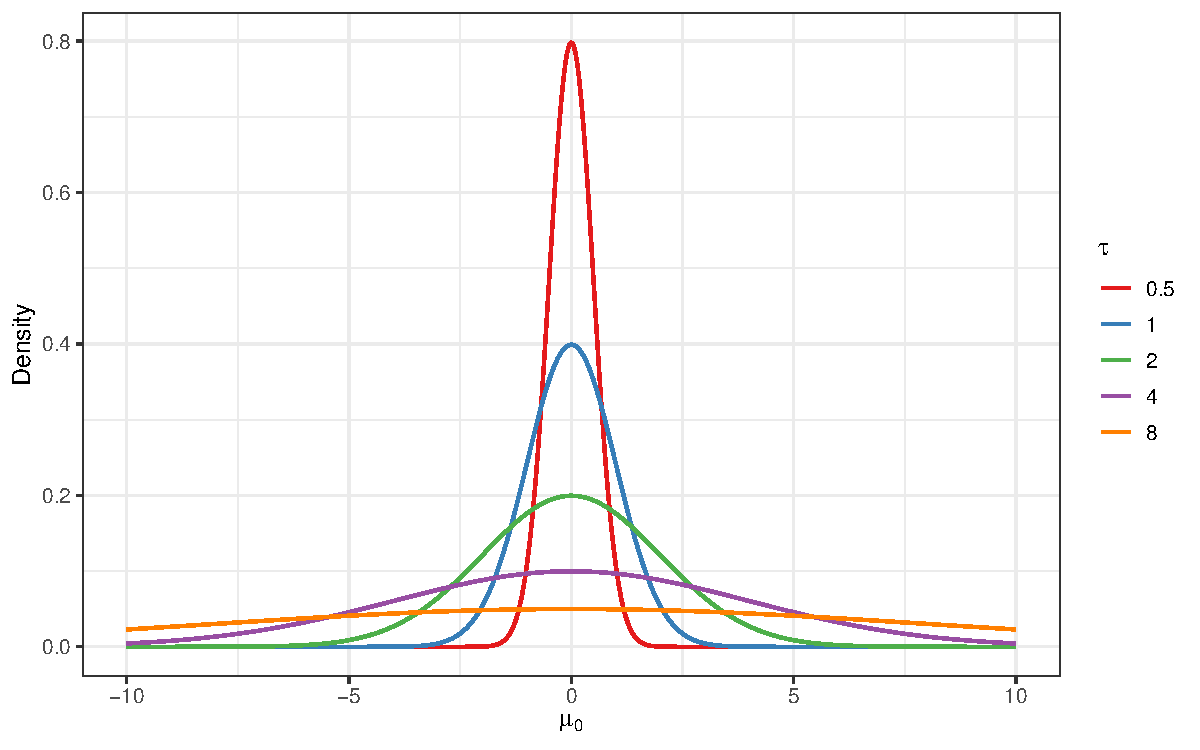
\includegraphics[keepaspectratio]{redefinenullhypothesis_stats_files/figure-pdf/fig-null-uncertainty-1.pdf}}

}

\caption{\label{fig-null-uncertainty}Null hypothesis with uncertainty:
\(\mu_0 = 0\), varying \(\tau\)}

\end{figure}%

\textbf{Notation.} Throughout this paper, we use two related uncertainty
parameters:

\begin{itemize}
\tightlist
\item
  \(\tau\): Uncertainty in the original measurement units
\item
  \(c\): Standardized uncertainty, defined as \(c = \tau/\sigma\)
\end{itemize}

Since the population mean \(\mu_0\) itself carries uncertainty, the
variance of \(\bar{X} - \mu_0\) becomes \(\sigma^2/n + \tau^2\). The
reformulated test statistic is:

\[z_{\tau} = \dfrac{\bar{X} - \mu_0}{\sqrt{\sigma^2/n + \tau^2}} \sim N(0,1)\]

\subsection{The Shrinkage Factor}\label{the-shrinkage-factor}

Substituting \(\tau = c\sigma\) yields:

\[z_{c\sigma} = \dfrac{\bar{X} - \mu_0}{\sqrt{\sigma^2/n + c^2\sigma^2}} = \dfrac{z}{\sqrt{1 + nc^2}}\]

This reveals that achieving statistical significance now requires a
z-value that is \(\sqrt{1 + nc^2}\) times larger than under traditional
hypothesis testing. Crucially, when \(c \neq 0\), we have:

\[|z_{c\sigma}| < \left|\frac{\bar{X} - \mu_0}{\tau}\right|\]

meaning that effects smaller than \(1.96 \times \tau\) can never achieve
\(p_{c\sigma} < 0.05\), regardless of sample size
(Figure~\ref{fig-p-shrinkage}).

\begin{figure}[H]

\centering{

\pandocbounded{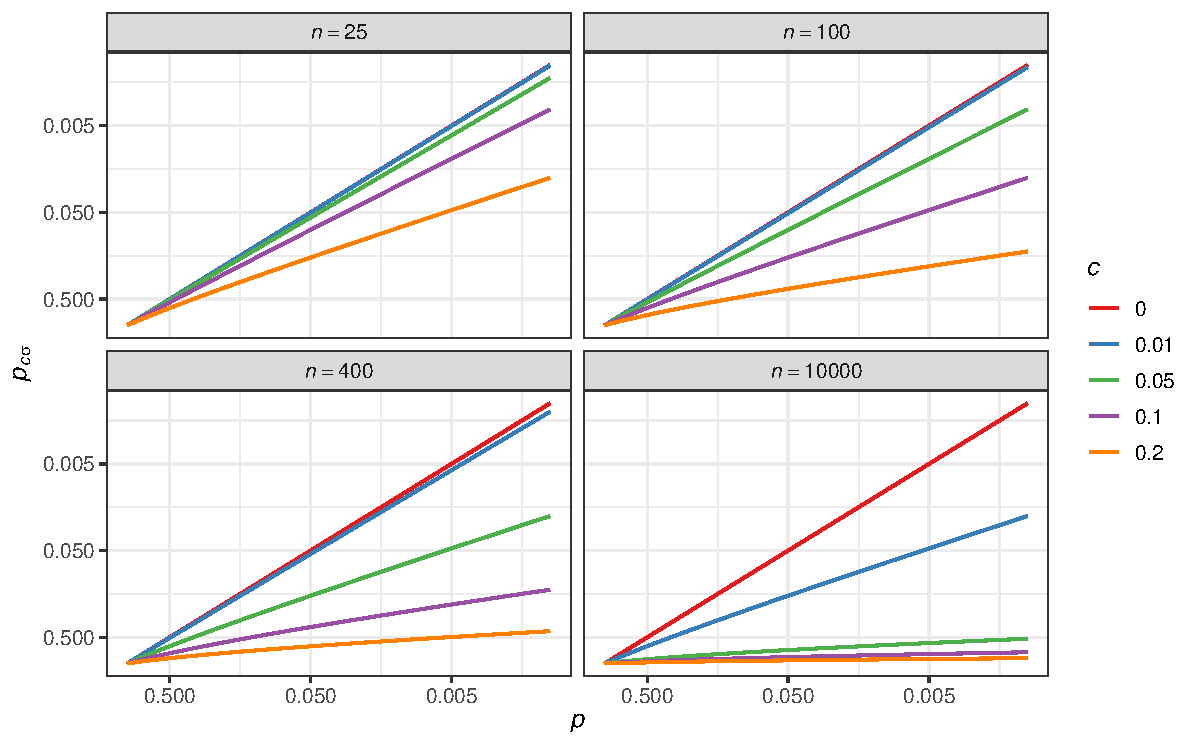
\includegraphics[keepaspectratio]{redefinenullhypothesis_stats_files/figure-pdf/fig-p-shrinkage-1.pdf}}

}

\caption{\label{fig-p-shrinkage}Effect-size-integrated \(p_{c\sigma}\)
across uncertainty (\(c\)) and sample size (\(n\))}

\end{figure}%

\subsection{Minimum Detectable Effect}\label{minimum-detectable-effect}

Expressing \(|z_{c\sigma}|\) in terms of effect size
\(d = |\bar{X} - \mu_0|/\sigma\) yields:

\[|z_{c\sigma}| = \dfrac{d}{\sqrt{1/n + c^2}}\]

For significance at level \(\alpha\), we require
\(|z_{c\sigma}| > z_{1-\alpha/2}\), giving:

\[\text{MDE}(n) = z_{1-\alpha/2} \cdot \sqrt{\frac{1}{n} + c^2}\]

As \(n \to \infty\),
\(\text{MDE} \to z_{1-\alpha/2} \cdot c \approx 1.96c\) (for
\(\alpha = 0.05\)). This provides a natural floor on detectable effects
(Figure~\ref{fig-mde}).

\begin{figure}[H]

\centering{

\pandocbounded{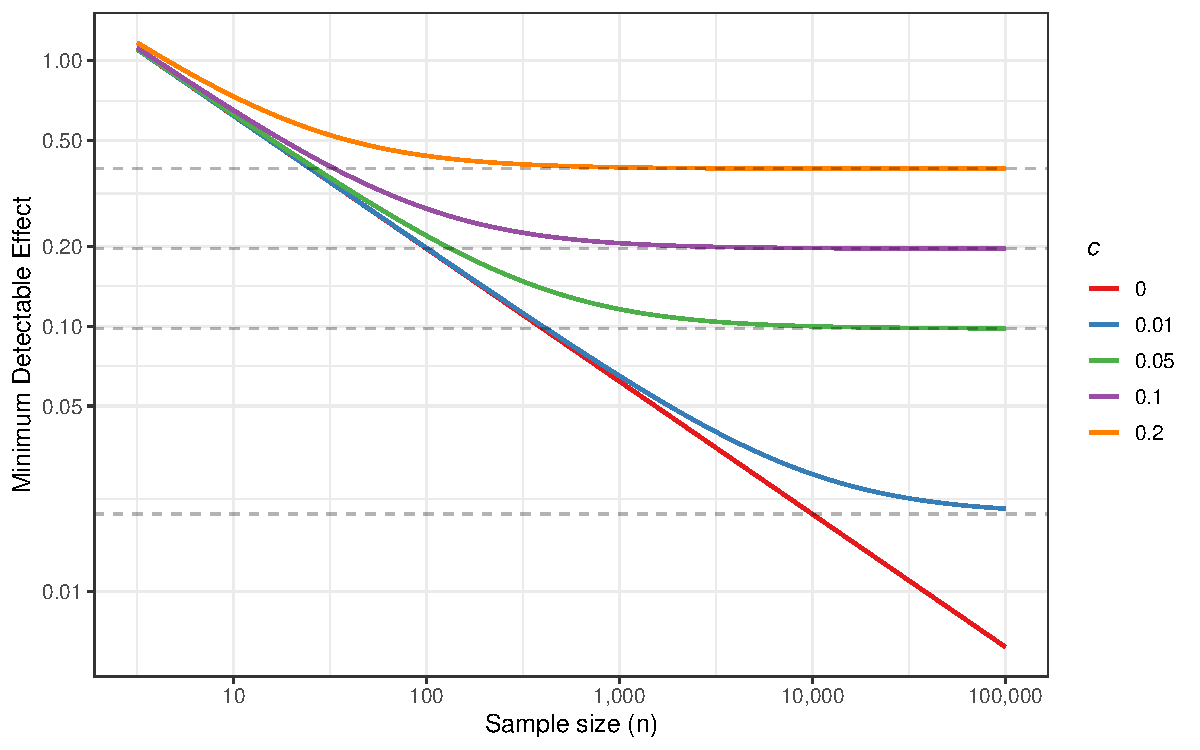
\includegraphics[keepaspectratio]{redefinenullhypothesis_stats_files/figure-pdf/fig-mde-1.pdf}}

}

\caption{\label{fig-mde}Minimum Detectable Effect (MDE) as a function of
sample size for different uncertainty levels}

\end{figure}%

\subsection{Extension to Other
Statistics}\label{extension-to-other-statistics}

\subsubsection{t-tests}\label{t-tests}

For one-sample and paired t-tests:
\[t_{cs} = \dfrac{t}{\sqrt{1 + nc^2}}\]

For independent two-sample t-tests (equal variance):
\[t_{cs_p} = \dfrac{t}{\sqrt{1 + \frac{n_1 n_2}{n_1 + n_2} c^2}}\]

\subsubsection{Regression Coefficients}\label{regression-coefficients}

For linear and generalized linear models:
\[z_{c} = \dfrac{z}{\sqrt{1 + nc^2}}\]

where \(z = \hat{\beta}/\text{se}(\hat{\beta})\) is the Wald statistic.

\textbf{Note on effective sample size.} In regression models with \(p\)
predictors, one may use the effective sample size
\(n_{\text{eff}} = n - p - 1\) (residual degrees of freedom) instead of
\(n\). For most practical purposes with moderate \(p/n\) ratios, using
\(n\) directly yields similar results.

\subsubsection{Welch t-test (Unequal
Variances)}\label{welch-t-test-unequal-variances}

The shrinkage principle extends naturally to the Welch t-test for
unequal variances. The same factor \(1/\sqrt{1 + n_{\text{eff}}c^2}\)
applies, where \(n_{\text{eff}}\) is computed from the
Welch-Satterthwaite approximation.

\subsubsection{General Formulation}\label{general-formulation}

For a Wald-type statistic \(W\) on the z or t scale, the
uncertainty-adjusted statistic and two-sided p-value are:
\[W_{c} = \frac{W}{\sqrt{1 + n_{\text{eff}} c^2}}, \quad p_{c\sigma} = 2\left(1 - F_{W}(|W_c|)\right)\]

where \(F_W\) is the standard normal or t distribution function.

For a chi-square Wald statistic
\(X^2 = \hat{\boldsymbol\theta}^\top \hat{V}^{-1} \hat{\boldsymbol\theta}\)
with \(k\) degrees of freedom, the statistic is already on a squared
scale, so the shrinkage factor enters squared. If the null uncertainty
is taken proportional to the sampling covariance,
\(\boldsymbol\theta \sim N(\mathbf{0},\, n_{\text{eff}} c^2 \hat{V})\),
then
\[X^2_{c} = \frac{X^2}{1 + n_{\text{eff}} c^2} \sim \chi^2_k, \quad p_{c\sigma} = 1 - F_{\chi^2_k}(X^2_c)\]

which uses only the upper tail. For \(k = 1\), \(X^2 = z^2\) and this
reduces exactly to the z-scale formula above.

\subsubsection{Connection to Confidence Intervals}\label{sec-ci}

The criterion \(|z_{c\sigma}| > z_{1-\alpha/2}\) is closely related to,
but not identical to, requiring that the \((1-\alpha)\) confidence
interval for the effect lies entirely outside the expanded null interval
\([-z_{1-\alpha/2} c\sigma, +z_{1-\alpha/2} c\sigma]\). On the
standardized scale, the interval criterion requires
\(d > z_{1-\alpha/2}(1/\sqrt{n} + c)\), whereas our criterion requires
\(d > z_{1-\alpha/2}\sqrt{1/n + c^2}\). Because
\(\sqrt{1/n + c^2} \le 1/\sqrt{n} + c\), the interval criterion is a
sufficient but more conservative condition; the two approximately
coincide when either \(1/\sqrt{n}\) or \(c\) dominates. This provides an
intuitive bridge to TOST and SGPV, which also rely on interval-based
reasoning.

\subsection{Use of Generative AI}\label{sec-ai}

Generative AI tools were used during the preparation of this manuscript
for TODO (tasks to be specified by the authors). All AI-assisted output
was reviewed and verified by the authors.

\section{Results}\label{sec-results}

\subsection{Simulation Study}\label{sec-sim}

\subsubsection{Type I Error Control}\label{type-i-error-control}

We evaluate the rejection rate of the uncertainty-adjusted test under
two data-generating processes: the conventional point null
(\(\mu = 0\)), and the distributional null from which the test is
derived, in which the true mean is drawn from \(N(0, c^2\sigma^2)\) in
each replicate (Table~\ref{tbl-type1}).

\begin{table}

\caption{\label{tbl-type1}Rejection rates of the uncertainty-adjusted
test at \(\alpha = 0.05\) under the point null and the distributional
null (10,000 simulations per scenario)}

\centering{

\begin{tabular}{cccccccc}
\toprule
\multicolumn{1}{c}{ } & \multicolumn{4}{c}{Point null ($\mu = 0$)} & \multicolumn{3}{c}{Distributional null ($\mu \sim N(0, c^2\sigma^2)$)} \\
\cmidrule(l{3pt}r{3pt}){2-5} \cmidrule(l{3pt}r{3pt}){6-8}
$n$ & $c=0$ & $c=0.01$ & $c=0.05$ & $c=0.1$ & $c=0.01$ & $c=0.05$ & $c=0.1$\\
\midrule
30 & 0.054 & 0.053 & 0.045 & 0.025 & 0.049 & 0.050 & 0.048\\
100 & 0.050 & 0.049 & 0.028 & 0.006 & 0.051 & 0.052 & 0.049\\
500 & 0.051 & 0.046 & 0.003 & 0.000 & 0.052 & 0.054 & 0.052\\
1000 & 0.051 & 0.041 & 0.000 & 0.000 & 0.051 & 0.047 & 0.053\\
5000 & 0.047 & 0.018 & 0.000 & 0.000 & 0.049 & 0.052 & 0.049\\
\bottomrule
\end{tabular}

}

\end{table}%

Under the distributional null, the rejection rate is close to the
nominal 0.05 for every combination of \(n\) and \(c\) (range
0.047--0.054), as expected from the derivation. Under the point null,
the rejection rate is at or below \(\alpha\) (up to Monte Carlo error,
SE \(\approx 0.002\)) and decreases with both \(n\) and \(c\); for
example, it is 0.003 at \(n = 500\) and \(c = 0.05\). The test therefore
controls the Type I error rate at or below \(\alpha\) and is
conservative under the point null. This conservativeness is intended:
when the true effect is exactly zero or negligible, the method should
rarely declare significance, and the protection grows with the sample
size. When \(c = 0\), the method reduces to the traditional z-test.

\subsubsection{Power Analysis}\label{power-analysis}

We compare the power of our method against traditional testing across
effect sizes (Figure~\ref{fig-power}).

\begin{figure}[H]

\centering{

\pandocbounded{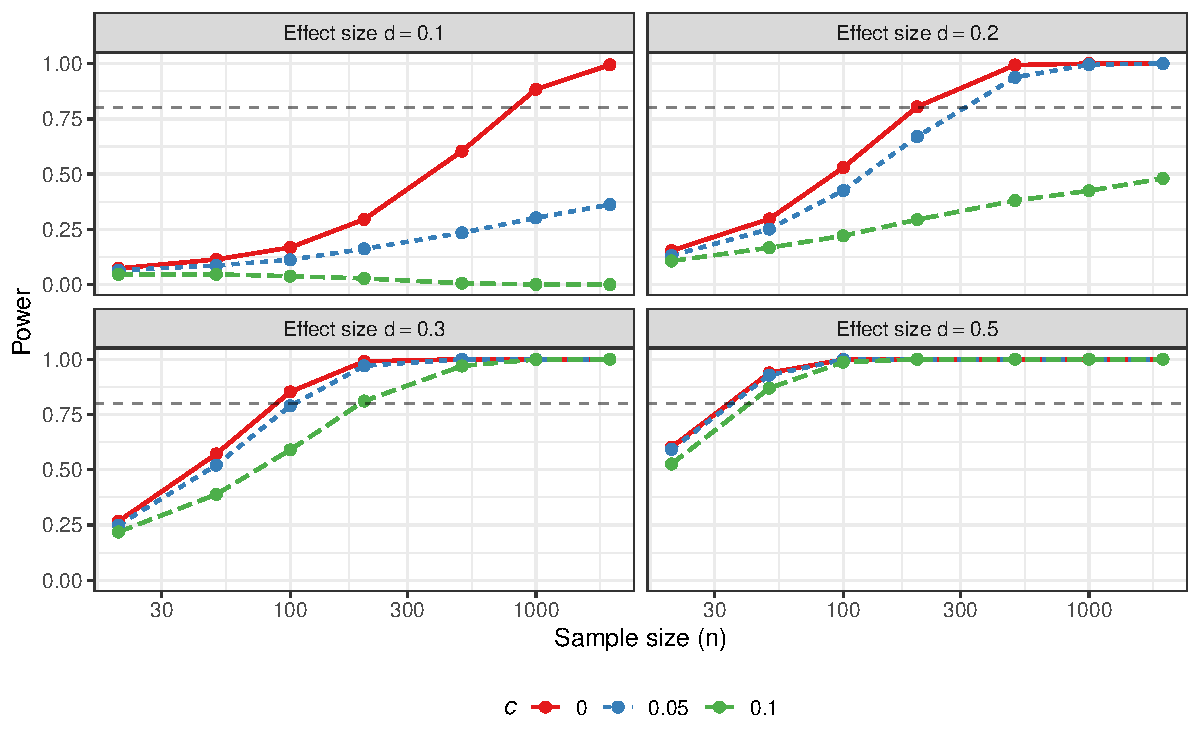
\includegraphics[keepaspectratio]{redefinenullhypothesis_stats_files/figure-pdf/fig-power-1.pdf}}

}

\caption{\label{fig-power}Power curves comparing traditional p-value and
uncertainty-adjusted \(p_{c\sigma}\) for various effect sizes}

\end{figure}%

Key observations:

\begin{enumerate}
\def\labelenumi{\arabic{enumi}.}
\tightlist
\item
  For small effect sizes (\(d = 0.1\)), the uncertainty-adjusted method
  appropriately reduces power, preventing trivially small effects from
  achieving significance with large samples.
\item
  For effects well above the asymptotic threshold \(1.96c\) (e.g.,
  \(d = 0.3\) or \(0.5\) with \(c \le 0.1\)), power approaches 1 as
  \(n\) increases, although more slowly than for the traditional test.
  For \(d = 0.2\) and \(c = 0.1\), the effect lies only slightly above
  \(1.96c = 0.196\), so power increases slowly.
\item
  The choice of \(c\) determines the effect size threshold: effects
  smaller than \(\approx 1.96c\) will never achieve significance
  regardless of sample size.
\end{enumerate}

\subsection{Real Data Application}\label{sec-real}

We demonstrate our method using the birthweight dataset from the MASS R
package (\citeproc{ref-venables2002mass}{Venables and Ripley 2002}),
originally described by Hosmer and Lemeshow
(\citeproc{ref-hosmer1989applied}{1989}), which contains data on 189
births at Baystate Medical Center, Springfield, MA during 1986. We
examine whether maternal smoking is associated with infant birth
weight---a well-established relationship in epidemiology
(Table~\ref{tbl-birthwt}).

\begin{table}

\caption{\label{tbl-birthwt}Effect of maternal smoking on birth weight:
Comparison of methods}

\centering{

\begin{threeparttable}
\begin{tabular}{llcl}
\toprule
Method & Null hypothesis & p-value & $H_0$ at $\alpha = 0.05$\\
\midrule
\addlinespace[0.3em]
\multicolumn{4}{l}{\textbf{Tests of difference}}\\
\hspace{1em}Traditional t-test & $\Delta = 0$ & 0.0087 & Rejected\\
\hspace{1em}Uncertainty-adjusted ($c = 0.1$) & $\Delta \sim N(0, c^2\sigma^2)$ & 0.0288 & Rejected\\
\hspace{1em}Uncertainty-adjusted ($c = 0.2$) & $\Delta \sim N(0, c^2\sigma^2)$ & 0.1146 & Not rejected\\
\hspace{1em}Uncertainty-adjusted ($c = 0.3$) & $\Delta \sim N(0, c^2\sigma^2)$ & 0.2394 & Not rejected\\
\addlinespace[0.3em]
\multicolumn{4}{l}{\textbf{Test of equivalence}}\\
\hspace{1em}TOST ($\delta = 0.2\sigma$) & $|\Delta| \ge \delta$ & 0.9042 & Not rejected\\
\bottomrule
\end{tabular}
\begin{tablenotes}
\item \textit{Note:} 
\item $\Delta$, true mean difference (non-smokers minus smokers); $\sigma$, pooled SD. TOST reverses the roles of the hypotheses: its null hypothesis is non-equivalence, so a small p-value supports equivalence. A large TOST p-value means that equivalence could not be established, not that a difference was shown.
\end{tablenotes}
\end{threeparttable}

}

\end{table}%

In this dataset, non-smoking mothers (\(n = 115\)) had a mean infant
birth weight of 3056 g (SD 753 g), and smoking mothers (\(n = 74\)) had
a mean of 2772 g (SD 660 g). The mean difference was 284 g (pooled SD
718 g), corresponding to Cohen's \(d = 0.395\) and \(t = 2.65\).

\textbf{Interpretation:} The traditional t-test yields a statistically
significant result (\(p = 0.009\)), indicating that infants of
non-smoking mothers weigh more than those of smoking mothers. The
observed effect size (\(d = 0.395\)) corresponds to a difference of
approximately 284 g. Because the sample is modest (effective sample size
\(n_1 n_2/(n_1+n_2) \approx 45\)), the finite-sample MDE is considerably
larger than its asymptotic floor \(1.96c\). With \(c = 0.1\)
(\(\mathrm{MDE} \approx 0.352\)), significance is maintained
(\(p_{c\sigma} = 0.029\)). With \(c = 0.2\)
(\(\mathrm{MDE} \approx 0.489\)), the observed effect falls below the
threshold and the result is no longer significant
(\(p_{c\sigma} = 0.115\)); the same holds for \(c = 0.3\)
(\(\mathrm{MDE} \approx 0.657\), \(p_{c\sigma} = 0.239\)). The TOST
p-value (0.904) answers a different question: it indicates that
equivalence within \(\pm 0.2\sigma\) could not be established, which is
why it is reported separately in Table~\ref{tbl-birthwt}. This example
illustrates how the choice of \(c\) encodes the researcher's judgment
about clinically meaningful effect sizes, and that in small samples the
evidence required for significance is stricter than the asymptotic
threshold alone suggests.

\subsection{Comparison with Equivalence Testing}\label{sec-tost}

TOST and the proposed test both replace the point null with a region of
practically negligible effects, but they ask opposite questions. TOST
takes non-equivalence (\(|\Delta| \ge \delta\)) as the null hypothesis
and seeks evidence that the effect is small, whereas the
uncertainty-adjusted test takes a negligible effect as the null
hypothesis and seeks evidence that the effect is large enough to matter.
To compare them on a common scale, we set \(\delta = 0.2\) and
\(c = 0.1\), so that the asymptotic threshold \(1.96c \approx 0.196\)
matches the equivalence bound. Figure~\ref{fig-comparison-tost} shows,
for two-sample comparisons with equal allocation, the rejection rate of
the traditional test, the rejection rate of the uncertainty-adjusted
test, and the rate at which TOST establishes equivalence, for total
sample sizes of 200 and 2,000 (3,000 replicates per scenario).

\begin{figure}[H]

\centering{

\pandocbounded{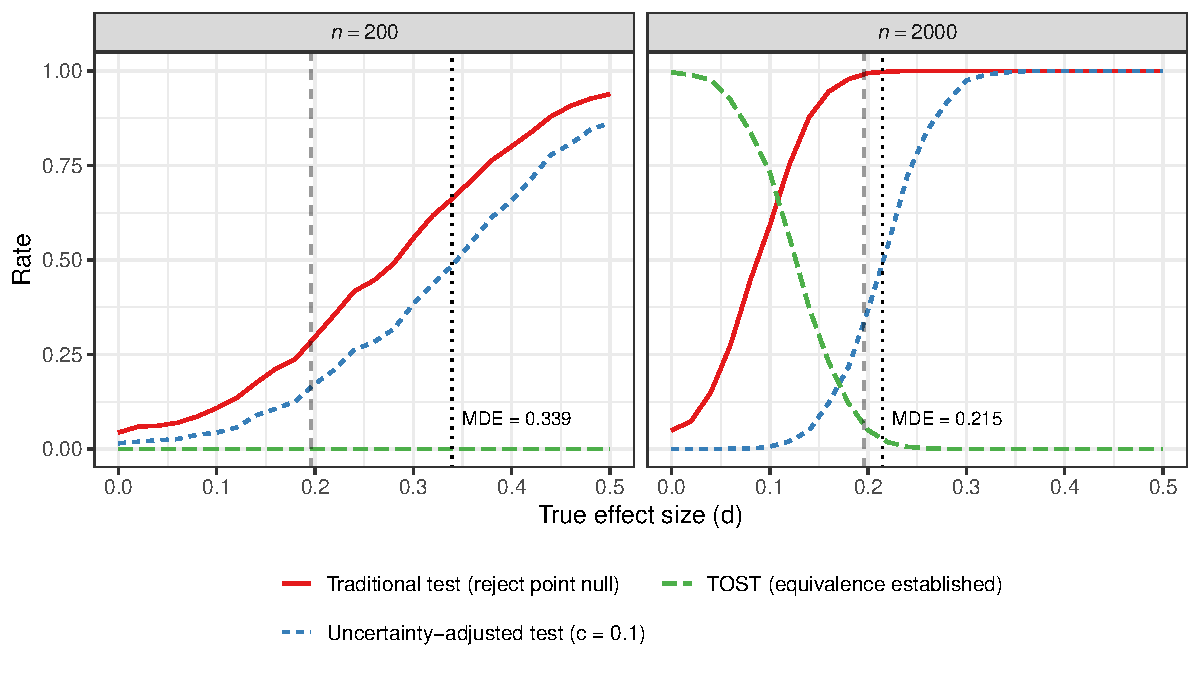
\includegraphics[keepaspectratio]{redefinenullhypothesis_stats_files/figure-pdf/fig-comparison-tost-1.pdf}}

}

\caption{\label{fig-comparison-tost}Traditional test,
uncertainty-adjusted test (\(c = 0.1\)), and TOST equivalence
(\(\delta = 0.2\)) across true effect sizes for total sample sizes of
200 and 2,000. Dotted lines mark the finite-sample MDE of the
uncertainty-adjusted test; dashed lines mark the asymptotic threshold
\(1.96c\).}

\end{figure}%

With \(n = 200\), the half-width of the 90\% confidence interval for the
mean difference (about 0.23 SD) exceeds the equivalence bound, so TOST
almost never establishes equivalence, even when the true effect is zero.
The uncertainty-adjusted test rejects only for effects well above the
bound, reaching about 50\% power near its finite-sample MDE (0.339).
Neither method supports a firm conclusion for effects between zero and
about 0.3, which reflects the limited information in a sample of this
size.

With \(n = 2{,}000\), the three procedures divide the effect-size axis
into distinct regions. For true effects near zero, TOST establishes
equivalence with high probability (1.00 at \(d = 0\)). For effects
between roughly 0.1 and 0.2, the traditional test rejects frequently
(0.88 at \(d = 0.14\)), whereas the uncertainty-adjusted test rarely
does (0.05); these differences are statistically detectable but fall
below the threshold of practical importance. For effects of about 0.3 or
larger, the uncertainty-adjusted test rejects with high probability
(0.97 at \(d = 0.3\)).

The uncertainty-adjusted test therefore behaves like a one-step
minimum-effect test. Its threshold, \(z_{1-\alpha/2}\sqrt{1/n + c^2}\),
combines sampling error and null uncertainty in quadrature, whereas the
interval criterion combines them additively (Section~\ref{sec-ci}). It
does not replace TOST: when the goal is to show that an effect is
negligible, an equivalence test is still required, and the two
procedures can be reported together.

\section{Practical Guidelines}\label{sec-guidelines}

\subsection{\texorpdfstring{Choosing the Uncertainty Parameter
\(c\)}{Choosing the Uncertainty Parameter c}}\label{choosing-the-uncertainty-parameter-c}

The choice of \(c\) should be guided by the minimum
clinically/practically important difference (MCID).
Table~\ref{tbl-guidelines} lists suggested values of \(c\) for several
minimum important effect sizes, together with the corresponding
asymptotic MDE.

\begin{table}

\caption{\label{tbl-guidelines}Recommended uncertainty parameter \(c\)
based on minimum important effect size. The Example column gives
illustrative examples only.}

\centering{

\begin{tabular}{cccl}
\toprule
Minimum important effect ($d$) & $c$ & MDE ($n \to \infty$) & Example\\
\midrule
0.02 & 0.010 & 0.020 & Large epidemiological studies\\
0.05 & 0.025 & 0.049 & Biomarker studies\\
0.10 & 0.050 & 0.098 & Standard clinical trials\\
0.20 & 0.100 & 0.196 & Behavioral interventions\\
0.30 & 0.150 & 0.294 & Strong treatment effects\\
\bottomrule
\end{tabular}

}

\end{table}%

\textbf{Rule of thumb:} Set \(c\) slightly below half the minimum
important effect size. This ensures that effects below your threshold
cannot achieve significance regardless of sample size, while effects
above it can be detected with adequate power.

\subsection{Sample Size Calculation}\label{sec-samplesize}

Under the alternative, the estimated standardized effect is
approximately \(N(d, 1/n)\), so its standard deviation is
\(\sqrt{1/n}\); the null uncertainty \(c\) enters only the rejection
threshold \(z_{1-\alpha/2}\sqrt{1/n + c^2}\). Ignoring the probability
of rejection in the opposite tail, the required sample size for power
\(1-\beta\) satisfies

\[d = z_{1-\alpha/2}\sqrt{\frac{1}{n} + c^2} + z_{1-\beta}\sqrt{\frac{1}{n}}.\]

Writing \(s = 1/\sqrt{n}\) and \(A = z_{1-\alpha/2}^2 - z_{1-\beta}^2\)
(positive whenever \(z_{1-\alpha/2} > z_{1-\beta}\), e.g.,
\(\alpha = 0.05\) and power 0.8), squaring
\(d - z_{1-\beta}s = z_{1-\alpha/2}\sqrt{s^2 + c^2}\) gives
\(A s^2 + 2 d z_{1-\beta} s - (d^2 - z_{1-\alpha/2}^2 c^2) = 0\), whose
positive root is

\[s = \frac{-d z_{1-\beta} + \sqrt{d^2 z_{1-\beta}^2 + A\,(d^2 - z_{1-\alpha/2}^2 c^2)}}{A}, \qquad n_{c\sigma} = \frac{1}{s^2}.\]

When \(c = 0\), this reduces to the traditional formula
\(n = \left((z_{1-\alpha/2} + z_{1-\beta})/d\right)^2\). If
\(d \leq z_{1-\alpha/2}\,c\), no finite sample size can achieve the
desired power---the target effect does not exceed the asymptotic minimum
detectable effect. Figure~\ref{fig-samplesize} shows the required sample
size for several values of \(c\).

\begin{figure}[H]

\centering{

\pandocbounded{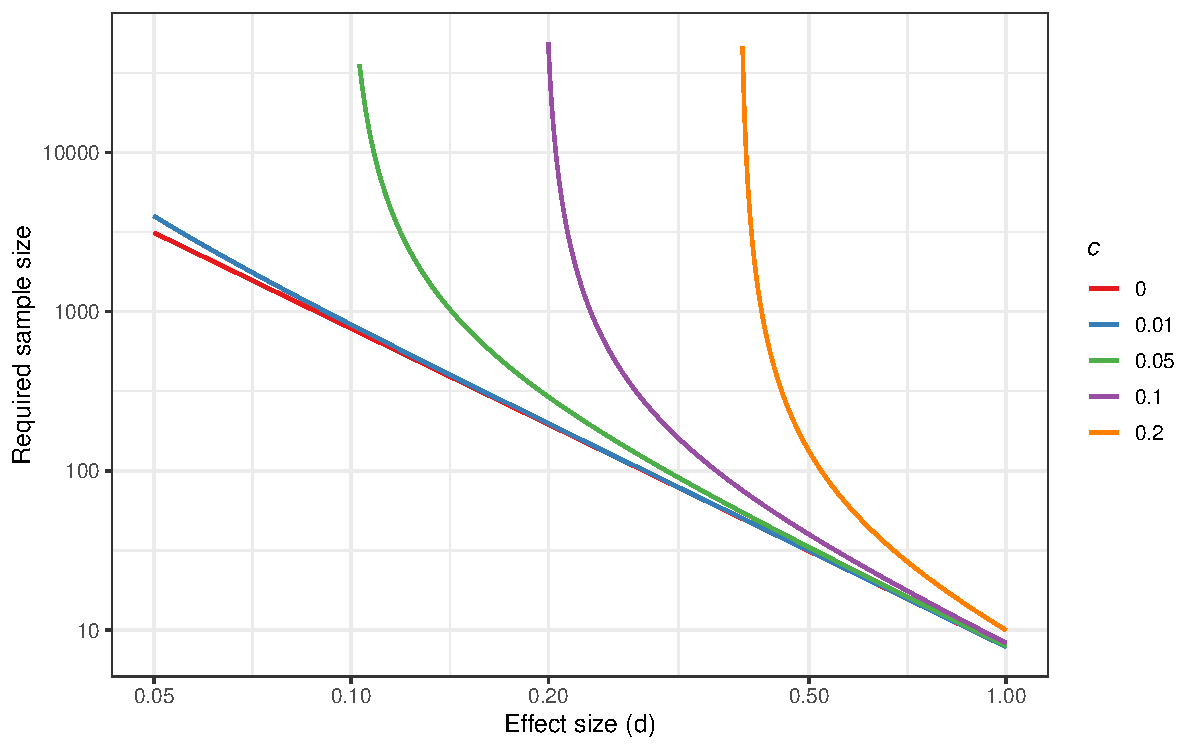
\includegraphics[keepaspectratio]{redefinenullhypothesis_stats_files/figure-pdf/fig-samplesize-1.pdf}}

}

\caption{\label{fig-samplesize}Required sample size with uncertainty
adjustment (\(\alpha = 0.05\), power = 0.8)}

\end{figure}%

\section{Discussion}\label{sec-discussion}

\subsection{Relation to Bayesian
Approaches}\label{relation-to-bayesian-approaches}

The variance \(\sigma^2/n + \tau^2\) underlying \(z_\tau\) is the
variance of the prior predictive distribution of \(\bar{X}\) when
\(\mu \sim N(\mu_0, \tau^2)\), and \(p_{c\sigma}\) is formally a prior
predictive p-value in the sense of Box
(\citeproc{ref-box1980sampling}{Box 1980}). The proposed test is
therefore identical in form to a Bayesian model check of a normal prior.
The two differ in interpretation and purpose. In the Bayesian setting,
\(\tau\) expresses prior belief about the parameter, the prior is
combined with the likelihood to form a posterior, and inference is based
on that posterior. In our framework, \(\tau\) is not a statement of
belief about where the parameter lies; it specifies how far from
\(\mu_0\) an effect may lie and still be regarded as practically
negligible, and it is chosen on substantive grounds
(Section~\ref{sec-guidelines}) rather than elicited as a prior. No
posterior is computed, and the resulting p-value is used in the usual
frequentist way, as a tail probability compared with a fixed threshold.
This view also clarifies the link to Lindley's paradox
(\citeproc{ref-lindley1957statistical}{Lindley 1957}): once
\(\tau > 0\), the test statistic for a fixed observed effect size
converges to \(d/c\) rather than growing without bound as \(n\)
increases, which removes the large-sample conflict that arises under a
point null.

\subsection{Advantages of the Proposed
Framework}\label{advantages-of-the-proposed-framework}

\begin{enumerate}
\def\labelenumi{\arabic{enumi}.}
\item
  \textbf{Unified framework:} Effect size and statistical significance
  are integrated into a single measure, eliminating the need to examine
  them separately.
\item
  \textbf{Sample-size adaptation:} Unlike fixed significance thresholds,
  our method naturally becomes more stringent as sample sizes grow large
  enough to detect trivially small effects.
\item
  \textbf{Transparency:} Researchers must explicitly specify their
  uncertainty parameter \(c\), forcing consideration of what effect
  sizes are practically meaningful.
\item
  \textbf{Compatibility:} The framework extends naturally to all
  Wald-type statistics (t-tests, regression coefficients, etc.).
\end{enumerate}

\subsection{Exploratory Extension: Multiple
Testing}\label{exploratory-extension-multiple-testing}

Testing many hypotheses at once can be viewed as increasing the
uncertainty attached to each null hypothesis. A natural extension is to
let the uncertainty grow with the number of hypotheses,
\(c_m = c \cdot m^b\), instead of shrinking \(\alpha\) as in Bonferroni
correction. With \(c = 0.01\) and \(b = 0.069\), this rule matches the
Bonferroni threshold at \(m = 10^6\) and \(n = 10{,}000\), a
configuration typical of genome-wide association studies
(Figure~\ref{fig-multiple}).

\begin{figure}[H]

\centering{

\pandocbounded{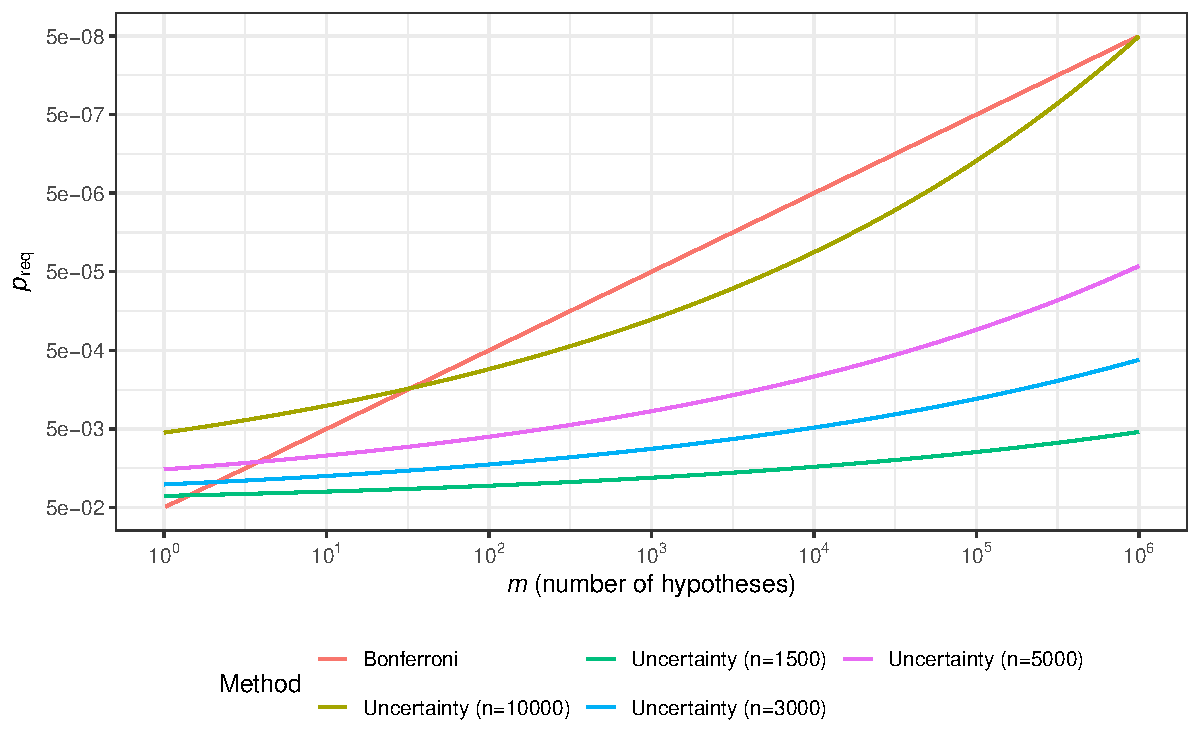
\includegraphics[keepaspectratio]{redefinenullhypothesis_stats_files/figure-pdf/fig-multiple-1.pdf}}

}

\caption{\label{fig-multiple}Required p-value (\(p_{\text{req}}\)) by
number of hypotheses (\(m\)): uncertainty control
(\(c_m = c \cdot m^b\), \(c = 0.01\), \(b = 0.069\)) at several sample
sizes vs Bonferroni correction}

\end{figure}%

At smaller sample sizes, however, the required p-value is far less
stringent than the Bonferroni threshold (about \(5.5 \times 10^{-3}\) at
\(n = 1{,}500\) and \(m = 10^6\), compared with \(5 \times 10^{-8}\)).
Under the global point null, the rule therefore does not control the
family-wise error rate, and the expected number of false positives can
be large when \(n\) is small. We regard uncertainty control as an
exploratory extension rather than a replacement for FWER or FDR control.
Characterizing its error-rate properties, for example the rate at which
effects smaller than \(1.96c_m\) are declared significant, and choosing
\(b\) in a principled way are left for future work.

\subsection{Limitations}\label{limitations}

\begin{enumerate}
\def\labelenumi{\arabic{enumi}.}
\item
  \textbf{Parameter selection:} The choice of \(c\) requires domain
  expertise and may be debated. We recommend sensitivity analyses across
  plausible \(c\) values.
\item
  \textbf{Not a complete solution:} This method addresses one limitation
  of p-values (sensitivity to sample size for trivial effects) but does
  not solve all problems with null hypothesis significance testing.
\item
  \textbf{Clustered/dependent data:} When observations are not
  independent (e.g., repeated measures, hierarchical data), the
  effective sample size differs from the total number of observations.
  For GEE or mixed models, consider using the number of independent
  clusters or an appropriate effective sample size rather than total
  \(n\).
\item
  \textbf{Novel approach:} As a relatively new method (first documented
  in 2018), more empirical evaluation across diverse applications is
  needed.
\end{enumerate}

\section{Conclusions}\label{sec-conclusion}

We have presented a redefined hypothesis testing framework that
incorporates uncertainty into the null hypothesis. By acknowledging that
point null hypotheses are unrealistic, our method provides
effect-size-integrated p-values that prevent trivially small differences
from achieving statistical significance. The test has exact size under
the distributional null and is conservative under the point null, while
providing researchers with a principled tool to distinguish between
statistical and practical significance.

The minimum detectable effect
\(\text{MDE}(n) = z_{1-\alpha/2}\sqrt{1/n + c^2}\) provides a natural
floor on detectable effects. Letting the uncertainty grow with the
number of hypotheses (\(c_m = c \cdot m^b\)) is a possible extension to
multiple testing whose error-rate properties remain to be established.

We encourage researchers to adopt this framework alongside traditional
analyses, particularly in large-sample studies where the distinction
between statistical and practical significance is most critical.

\begin{center}\rule{0.5\linewidth}{0.5pt}\end{center}

\emph{This work was originally conceived in 2017 and first publicly
documented on November 8, 2018 at
https://blog.zarathu.com/posts/2018-11-08-redefinenullhypothesis/}

\textbf{Supplementary Materials:} The following supporting information
can be downloaded at: TODO (link assigned by the journal). Code S1: R
scripts reproducing all simulations, tables, and figures.

\textbf{Author Contributions:} Conceptualization, J.K.; methodology,
J.K. and T.S.; software, T.S.; validation, T.S.; formal analysis, J.K.
and T.S.; writing---original draft preparation, J.K.; writing---review
and editing, J.K. and T.S.; visualization, T.S.; supervision, J.K. All
authors have read and agreed to the published version of the manuscript.

\textbf{Funding:} This research received no external funding.

\textbf{Data Availability Statement:} The birth weight data analyzed in
this study are publicly available as the dataset \texttt{birthwt} in the
R package MASS. The R code used to generate all simulation results,
tables, and figures is available at
\url{https://github.com/staehee/redefinenullhypothesis/tree/main/code}
and as Code S1 in the Supplementary Materials.

\textbf{Acknowledgments:} During the preparation of this manuscript, the
authors used {[}TODO: tool name, version{]} for the purposes of
{[}TODO{]}. The authors have reviewed and edited the output and take
full responsibility for the content of this publication.

\textbf{Conflicts of Interest:} The authors declare no conflicts of
interest.

\section*{References}\label{references}
\addcontentsline{toc}{section}{References}

\protect\phantomsection\label{refs}
\begin{CSLReferences}{1}{1}
\bibitem[\citeproctext]{ref-anderson2000null}
Anderson, David R., Kenneth P. Burnham, and William L. Thompson. 2000.
{``Null Hypothesis Testing: Problems, Prevalence, and an Alternative.''}
\emph{The Journal of Wildlife Management} 64 (4): 912--23.
\url{http://www.jstor.org/stable/3803199}.

\bibitem[\citeproctext]{ref-Benjamin2018}
Benjamin, Daniel J., James O. Berger, Magnus Johannesson, et al. 2018.
{``Redefine Statistical Significance.''} \emph{Nature Human Behaviour} 2
(1): 6--10. \url{https://doi.org/10.1038/s41562-017-0189-z}.

\bibitem[\citeproctext]{ref-blume2018second}
Blume, Jeffrey D, Lucy D'Agostino McGowan, William D Dupont, and Robert
A Greevy Jr. 2018. {``Second-Generation p-Values: Improved Rigor,
Reproducibility, \& Transparency in Statistical Analyses.''} \emph{PloS
One} 13 (3): e0188299.
\url{https://doi.org/10.1371/journal.pone.0188299}.

\bibitem[\citeproctext]{ref-box1980sampling}
Box, George E. P. 1980. {``Sampling and {Bayes}' Inference in Scientific
Modelling and Robustness.''} \emph{Journal of the Royal Statistical
Society: Series A (General)} 143 (4): 383--430.
\url{https://doi.org/10.2307/2982063}.

\bibitem[\citeproctext]{ref-cohen1994earth}
Cohen, Jacob. 1994. {``The Earth Is Round (\(p < .05\)).''}
\emph{American Psychologist} 49 (12): 997--1003.
\url{https://doi.org/10.1037/0003-066X.49.12.997}.

\bibitem[\citeproctext]{ref-hodges1954testing}
Hodges, J. L., and E. L. Lehmann. 1954. {``Testing the Approximate
Validity of Statistical Hypotheses.''} \emph{Journal of the Royal
Statistical Society: Series B (Methodological)} 16 (2): 261--68.
\url{https://doi.org/10.1111/j.2517-6161.1954.tb00169.x}.

\bibitem[\citeproctext]{ref-hosmer1989applied}
Hosmer, David W., and Stanley Lemeshow. 1989. \emph{Applied Logistic
Regression}. 1st ed. Wiley.

\bibitem[\citeproctext]{ref-jama20181536}
Ioannidis, John P. A. 2018. {``The Proposal to Lower p Value Thresholds
to .005.''} \emph{JAMA} 319 (14): 1429--30.
\url{https://doi.org/10.1001/jama.2018.1536}.

\bibitem[\citeproctext]{ref-kruschke2018bayesian}
Kruschke, John K, and Torrin M Liddell. 2018. {``The Bayesian New
Statistics: Hypothesis Testing, Estimation, Meta-Analysis, and Power
Analysis from a Bayesian Perspective.''} \emph{Psychonomic Bulletin \&
Review} 25 (1): 178--206.
\url{https://doi.org/10.3758/s13423-016-1221-4}.

\bibitem[\citeproctext]{ref-lakens2017equivalence}
Lakens, Daniël. 2017. {``Equivalence Tests: A Practical Primer for t
Tests, Correlations, and Meta-Analyses.''} \emph{Social Psychological
and Personality Science} 8 (4): 355--62.
\url{https://doi.org/10.1177/1948550617697177}.

\bibitem[\citeproctext]{ref-lin2013too}
Lin, Mingfeng, Henry C. Lucas, and Galit Shmueli. 2013. {``Too Big to
Fail: Large Samples and the \(p\)-Value Problem.''} \emph{Information
Systems Research} 24 (4): 906--17.
\url{https://doi.org/10.1287/isre.2013.0480}.

\bibitem[\citeproctext]{ref-lindley1957statistical}
Lindley, D. V. 1957. {``A Statistical Paradox.''} \emph{Biometrika} 44
(1/2): 187--92. \url{https://doi.org/10.1093/biomet/44.1-2.187}.

\bibitem[\citeproctext]{ref-meehl1967theory}
Meehl, Paul E. 1967. {``Theory-Testing in Psychology and Physics: A
Methodological Paradox.''} \emph{Philosophy of Science} 34 (2): 103--15.
\url{https://doi.org/10.1086/288135}.

\bibitem[\citeproctext]{ref-sullivan2012using}
Sullivan, Gail M, and Richard Feinn. 2012. {``Using Effect Size---or Why
the p Value Is Not Enough.''} \emph{Journal of Graduate Medical
Education} 4 (3): 279--82.
\url{https://doi.org/10.4300/JGME-D-12-00156.1}.

\bibitem[\citeproctext]{ref-venables2002mass}
Venables, William N, and Brian D Ripley. 2002. \emph{Modern Applied
Statistics with {S}}. 4th ed. Springer.
\url{https://www.stats.ox.ac.uk/pub/MASS4/}.

\bibitem[\citeproctext]{ref-ronald2016asa}
Wasserstein, Ronald L., and Nicole A. Lazar. 2016. {``The ASA's
Statement on p-Values: Context, Process, and Purpose.''} \emph{The
American Statistician} 70 (2): 129--33.
\url{https://doi.org/10.1080/00031305.2016.1154108}.

\bibitem[\citeproctext]{ref-2528399}
Yates, F. 1964. {``Sir Ronald Fisher and the Design of Experiments.''}
\emph{Biometrics} 20 (2): 307--21.
\url{http://www.jstor.org/stable/2528399}.

\end{CSLReferences}




\end{document}
